\documentclass{article}
\usepackage[utf8]{inputenc}
\usepackage[margin=2cm]{geometry}
%\usepackage{enumitem}
\usepackage{csquotes}

% maths packages
\usepackage{amsmath}
\usepackage{amssymb}
\usepackage{amsthm}

% graphics packages
\usepackage{graphicx}
%\usepackage{subfig}
\usepackage[font={small,it}]{caption}
\usepackage{tikz}
\usetikzlibrary{positioning, circuits.logic.US}

\title{Constant Bernoulli Factories}
\author{Suzie Brown}
\date{\today}

% bibliography
\usepackage[round, sort&compress]{natbib}
\usepackage{har2nat} %%% Harvard reference style
\bibliographystyle{agsm}

% theorems
\newtheorem{thm}{Theorem}
\theoremstyle{definition}
\newtheorem{defn}{Definition}
\newtheorem{example}{Example}

% probability symbols
\newcommand{\PR}{\mathbb{P}}
\newcommand{\E}{\mathbb{E}}
\newcommand{\V}{\operatorname{Var}}
\newcommand{\iidsim}{\overset{iid}{\sim}}
\newcommand{\eqdist}{\overset{d}{=}}

% distributions
\newcommand{\Bern}{\operatorname{Bernoulli}}
\newcommand{\Geom}{\operatorname{Geom}}

% project-specific commands
\newcommand{\A}{\mathcal{A}}
\newcommand{\AND}{{\footnotesize AND }}
\newcommand{\NAND}{{\footnotesize NAND }}
\newcommand{\OR}{{\footnotesize OR }}
\newcommand{\NOR}{{\footnotesize NOR }}
\newcommand{\NOT}{{\footnotesize NOT }}

\begin{document}
\section{Strategies for constant Bernoulli factories}
By the definition of \citet{keane1994}, any constant function (i.e.\ independent of $p$) is \emph{simulable}, because we can ignore the $p$-coins altogether and simply use an auxiliary random variable. In particular, for any $c\in[0,1]$, we can sample a random variable $u \sim U(0,1)$ and output heads iff $u < c$.

We will see later on that constant functions are also \emph{strongly simulable}; that is, they can be simulated from $p$-coins without the use of auxiliary random variables. We later reveal constant functions (with $c\in(0,1)$) to be a special case of the class of strongly simulable functions given by the Keane-O'Brien theorem \citep{keane1994}. But first we take a detour into how one might construct exact simulations of certain constants, as opposed to approximate simulations via Bernstein polynomials that are usually applied in the literature.

\subsection{A first na\"ive construction}
Let us consider first the Bernoulli factory described in \citet{vonneumann1951}, for the constant function $f(p)\equiv 1/2$:

\begin{displayquote}
\textit{To cite a human example, for simplicity, in tossing a coin it is probably easier to make two consecutive tosses independent than to toss heads with probability exactly one-half. If independence of successive tosses is assumed, we can reconstruct a 50-50 chance out of even a badly biased coin by tossing twice. If we get heads-heads or tails-tails, we reject the tosses and try again. If we get head-tails (or tails-heads), we accept the result as heads (or tails). The resulting process is rigorously unbiased, although the amended process is at most 25 percent as efficient as ordinary coin-tossing.}
\end{displayquote}
Most authors now use the slightly more convenient convention with the outcomes inverted, so that once 10 or 01 is observed, the output of the Bernoulli factory is equal to the last coin flip (0 or 1 respectively). 
It is easy to show that, as claimed, this procedure produces an output heads with probability 1/2:
\begin{equation*}
\PR(Y=1) = \PR(X_\tau = 1) = \PR(X_2 = 1 \mid X_2\neq X_1) = \frac{\PR(X_1 = 0, X_2 = 1)}{\PR(X_1 = 0, X_2 = 1) + \PR(X_1 = 1, X_2 = 0)} = \frac{p(1-p)}{2p(1-p)} = \frac{1}{2}.
\end{equation*}
The running time of this procedure is random, and indeed unbounded. In particular, $\tau \eqdist 2\times\Geom(2p(1-p))$, with expectation $\E(\tau) = \frac{1}{p(1-p)}$. Figure \ref{fig:runtime_const2} shows the expected running time for various values of $p$. The expected running time achieves its minimum value of four when $p=1/2$ (that is, the coin was already unbiased), hence von Neumann's claim that ``the amended process is at most 25 percent as efficient as ordinary coin-tossing'' (which has deterministic running time one). The expected running time approaches infinity when $p$ is close to 0 or 1, but is moderate across a large range non-extreme values.\\

\begin{figure}
\centering
\includegraphics[width=0.8\textwidth]{vonneu_runtime.pdf}
\caption{•}
\label{fig:runtime_const2}
\end{figure}

We can generalise von Neumann's procedure to produce Bernoulli factories for $f(p)\equiv 1/k$ with $k\in\{2,3,\dots\}$. We simply toss the $p$-coin $k$ times and, if the outcome is a sequence with one head and $k-1$ tails, we output the last coin flip in the sequence. Otherwise we start again.
Now the probability of observing a usable sequence is $p(1-p)^{k-1}$, which is (strictly if $p\in(0,1)$) decreasing in $k$, so the efficiency will be even worse than in the initial case $k=2$. The running time has distribution $\tau \eqdist k \times \Geom(kp(1-p)^{k-1})$.
But we can mitigate this slightly: a sequence with one tail and $k-1$ heads would also work, with the outputs inverted. So we need only wait for whichever of these sequences occurs first. Now the distribution of the running time is $\tau \eqdist k \times \min\{\Geom(kp(1-p)^{k-1}), \Geom(kp^{k-1}(1-p))\} \eqdist k \times \Geom(1- [1-kp(1-p)^{k-1}][1-kp^{k-1}(1-p)])$.

Figure \ref{fig:runtime_const3} shows the expected running time when $k=3$; when considering only sequences with two heads and a tail, or only sequences with two tails and a head, or whichever occurs first.
It is clear from the figure that this adjustment considerably improves the efficiency, particularly when $p$ is not close to 1/2. The expected running time is minimised at $p=1/2$, where it takes the value $\frac{64}{13} \simeq 4.9$. This is not much worse than the $f(p)=1/2$ Bernoulli factory, and the curves for $f(p)=1/2$ and $f(p)=1/3$ are at least this close everywhere.\\

\begin{figure}
\centering
\includegraphics[width=0.8\textwidth]{const3_runtime.pdf}
\caption{•}
\label{fig:runtime_const3}
\end{figure}

This is looking promising: here is a reasonably efficient procedure that can produce any function $f(p)\equiv 1/k$; or of course $f(p)\equiv (k-1)/k$ by inverting the outputs.
But there is a problem. Figures \ref{fig:runtime_const4} and \ref{fig:runtime_const8} show the expected running time for $k=4$ and $k=8$ respectively. As $k$ increases, the procedure quickly becomes inefficient for $p$ close to 1/2. At $k=4$ we see the first non-convex function, with two minima appearing --- at $p \simeq 0.30, 0.70$ with $\E(\tau) \simeq 8.77$. And by the time $k=8$ things have gone badly wrong. The minima are now at $p\simeq 0.125, 0.875$ with value $\E(\tau) \simeq 20.37$, but more importantly, the local maximum at $p=1/2$ is now a large peak with $\E(\tau) \simeq 130.0$. Alas, this na\"ive construction is not so efficient after all.

It is not surprising that, for larger $k$, the efficiency is high for moderately extreme values of $p$ but low for $p$ close to 1/2. This procedure requires us to observe $k-1$ tails (or heads) out of $k$ tosses, which is a rare event with an unbiased coin, but a likely one with a coin strongly biased towards tails or heads respectively.

Figures \ref{fig:runtime_const4} and \ref{fig:runtime_const8} also show the expected running time for an alternative procedure. A (1/4)-coin can be constructed from two (1/2) coins by outputting heads iff both coins output heads, and a (1/8)-coin can be constructed from three (1/2)-coins in the same way. Figure \ref{fig:runtime_const4} shows that with $k=4$ this alternative procedure is already more efficient for some values of $p$ close to 1/2, and with $k=8$ (Figure \ref{fig:runtime_const8}) the comparison is striking, although the alternative still doesn't do so well for extreme values of $p$.

\begin{figure}
\centering
\includegraphics[width=0.8\textwidth]{const4_runtime.pdf}
\caption{•}
\label{fig:runtime_const4}
\end{figure}

\begin{figure}
\centering
\includegraphics[width=0.8\textwidth]{const8_runtime.pdf}
\caption{•}
\label{fig:runtime_const8}
\end{figure}

\subsection{Constants as functions of (1/2)-coins}
We have mentioned how a ($1/2^{n}$)-coin can be constructed by combining the results of $n$ (1/2)-coins. We achieved this using an \AND operator, i.e.\ multiplying the outputs. It is easy to see that the set of functions constructible using only \AND operators on (1/2)-coins is indeed limited to $\{f(p)=2^{-n} \mid n\in\mathbb{N}\}$. But there are other logical operators at our disposal: it is well known in computer science that any logic circuit can be constructed using only {\footnotesize NAND} operators, so perhaps we could do much better if we made use of \NOT (inversion) operators too.

As an example, imagine we would like to construct a Bernoulli factory for $f(p)\equiv \frac{11}{16}$. Noting that \AND is equivalent to $\times$ and \NOT is equivalent to $1-$, we find the following decomposition.
\begin{align*}
\frac{11}{16} &= 1- \frac{5}{16} 
= 1 - \frac{1}{2} \times \frac{5}{8} \\
&= 1 - \frac{1}{2} \times \left(1 - \frac{3}{8}\right) 
= 1 - \frac{1}{2} \times \left(1 - \frac{1}{2} \times \frac{3}{4}\right) \\
&= 1 - \frac{1}{2} \times \left(1 - \frac{1}{2} \times \left(1-\frac{1}{4}\right)\right)
= 1 - \frac{1}{2} \times \left(1 - \frac{1}{2} \times \left(1-\frac{1}{2} \times \frac{1}{2}\right)\right)
\end{align*}
This can be represented as a logic circuit with four (1/2)-coins as inputs, as shown in Figure \ref{fig:const_circuit}.

\begin{figure}
\centering
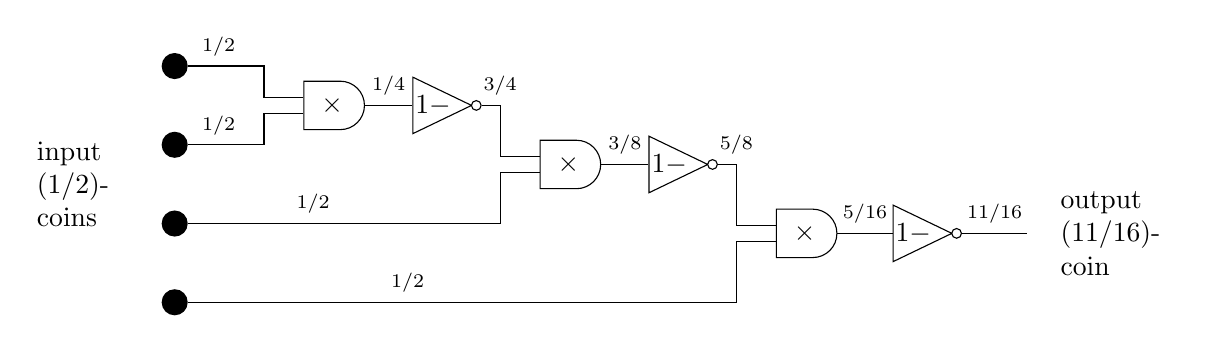
\begin{tikzpicture}[circuit logic US]
\node[circle, fill=black] at (0,0) (coin1) {} ;
\node[circle, fill=black] at (0,-1) (coin2) {} ;
\node[circle, fill=black] at (0,-2) (coin3) {} ;
\node[circle, fill=black] at (0,-3) (coin4) {} ;
\node[circle] at (11, -17/8) (output) {} ;

\node[and gate, draw, inputs={nn}] at (2,-1/2) (and1) {$\times$} ;
\node[not gate, draw, right = 0.6cm of and1] (not1) {$1-$} ;
\node[and gate, draw, inputs={nn}] at (5,-5/4) (and2) {$\times$} ;
\node[not gate, draw, right = 0.6cm of and2] (not2) {$1-$} ;
\node[and gate, draw, inputs={nn}] at (8, -17/8) (and3) {$\times$} ;
\node[not gate, draw, right = 0.7cm of and3] (not3) {$1-$} ;

\draw (and1.input 1) -- ++(left:5mm) |- node[above, pos=0.8]{\scriptsize 1/2} (coin1.east) ;
\draw (and1.input 2) -- ++(left:5mm) |- node[above, pos=0.8]{\scriptsize 1/2} (coin2.east) ;
\draw (and1.output) -- node[above]{\scriptsize 1/4} (not1.input) ;
\draw (and2.input 1) -- ++(left:5mm) |- node[above]{\scriptsize 3/4} (not1.output) ;
\draw (and2.input 2) -- ++(left:5mm) |- node[above, pos=0.8]{\scriptsize 1/2} (coin3.east) ;
\draw (and2.output) -- node[above]{\scriptsize 3/8} (not2.input) ;
\draw (and3.input 1) -- ++(left:5mm) |- node[above]{\scriptsize 5/8} (not2.output) ;
\draw (and3.input 2) -- ++(left:5mm) |- node[above, pos=0.8]{\scriptsize 1/2} (coin4.east) ;
\draw (and3.output) -- node[above]{\scriptsize 5/16} (not3.input) ;
\draw (not3.output) -- node[above]{\scriptsize 11/16} (output) ;

\node[text width = 1.5cm] at (-1,-3/2) (label1) {input (1/2)-coins} ;
\node[text width = 1.5cm] at (12,-17/8) (label2) {output (11/16)-coin} ;
\end{tikzpicture}
\caption{Logic circuit representation of an algorithm to produce one (11/16)-coin flip from four (1/2)-coin flips using \AND and \NOT gates}\label{fig:const_circuit}
\end{figure}

Because we are only using (1/2)-coins as inputs, and \NOT operators leave the denominator invariant while \AND operators multiply the denominators, this procedure can only produce constants that can be written as $k/2^n$. By the same arguments it can also be deduced that the number of (1/2)-coins required as inputs is always equal to $n$.
In fact, it is the case that any constant that can be written as $k/2^n$ (equivalently, having a terminating binary expansion) can be simulated by such a circuit, although this is not obvious.

Nonetheless, accepting this proposition, it is easy to show that any constant can therefore be approximately simulated to arbitrary precision, and that the approximation error decreases exponentially in the number of (1/2)-coins used. Given $c \in (0,1)$ and tolerance $\varepsilon$, we truncate the binary expansion of $c$ after $-\lfloor\log_2(\varepsilon)\rfloor -1$ places, and write the resulting constant as a fraction. This fraction will necessarily be of the form $k/2^n$, with $n\leq -\lfloor\log_2(\varepsilon)\rfloor -1$, and the approximation error is bounded by $|c-(k/2^n)| \leq 2^{-n-1} \leq 2^{\lfloor\log_2(\varepsilon)\rfloor} \leq \varepsilon$.
By our proposition, this fraction can be simulated using at most $-\lfloor\log_2(\varepsilon)\rfloor -1$ queries of a (1/2)-coin. Therefore truncating the binary expansion of $c$ to one more place decreases the approximation error by a factor of 2, and we conclude that the approximation error decreases exponentially in the number of (1/2)-coins used.

It is also possible to construct the same class of constants using a combination of \OR and \NOT operators. Figure \ref{fig:const_circuit2} shows the logic circuit representing a decomposition of the same constant 11/16 using \OR operators instead of \AND operators. Although the \OR gates are labelled $+$, this is a logical addition and doesn't correspond to a mathematical addition in the way \AND corresponds to $\times$.
The number of inputs is the same as for the \AND circuit, for the same reasons, and so the same result holds regarding the scaling of the approximation error for constants that can't be simulated exactly.

\begin{figure}
\centering
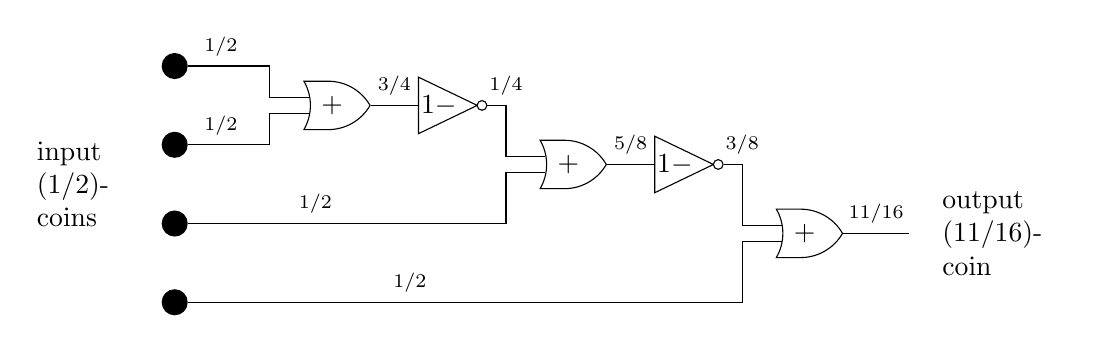
\begin{tikzpicture}[circuit logic US]
\node[circle, fill=black] at (0,0) (coin1) {} ;
\node[circle, fill=black] at (0,-1) (coin2) {} ;
\node[circle, fill=black] at (0,-2) (coin3) {} ;
\node[circle, fill=black] at (0,-3) (coin4) {} ;
\node[circle] at (9.5, -17/8) (output) {} ;

\node[or gate, draw, inputs={nn}] at (2,-1/2) (or1) {$+$} ;
\node[not gate, draw, right = 0.6cm of or1] (not1) {$1-$} ;
\node[or gate, draw, inputs={nn}] at (5,-5/4) (or2) {$+$} ;
\node[not gate, draw, right = 0.6cm of or2] (not2) {$1-$} ;
\node[or gate, draw, inputs={nn}] at (8, -17/8) (or3) {$+$} ;

\draw (or1.input 1) -- ++(left:5mm) |- node[above, pos=0.8]{\scriptsize 1/2} (coin1.east) ;
\draw (or1.input 2) -- ++(left:5mm) |- node[above, pos=0.8]{\scriptsize 1/2} (coin2.east) ;
\draw (or1.output) -- node[above]{\scriptsize 3/4} (not1.input) ;
\draw (or2.input 1) -- ++(left:5mm) |- node[above]{\scriptsize 1/4} (not1.output) ;
\draw (or2.input 2) -- ++(left:5mm) |- node[above, pos=0.8]{\scriptsize 1/2} (coin3.east) ;
\draw (or2.output) -- node[above]{\scriptsize 5/8} (not2.input) ;
\draw (or3.input 1) -- ++(left:5mm) |- node[above]{\scriptsize 3/8} (not2.output) ;
\draw (or3.input 2) -- ++(left:5mm) |- node[above, pos=0.8]{\scriptsize 1/2} (coin4.east) ;
\draw (or3.output) -- node[above]{\scriptsize 11/16} (output) ;

\node[text width = 1.5cm] at (-1,-3/2) (label1) {input (1/2)-coins} ;
\node[text width = 1.5cm] at (10.5,-17/8) (label2) {output (11/16)-coin} ;
\end{tikzpicture}
\caption{Logic circuit representation of an algorithm to produce one (11/16)-coin flip from four (1/2)-coin flips using \OR and \NOT gates}\label{fig:const_circuit2}
\end{figure}

The principle in computer science states that any logic circuit can be decomposed into only \NAND or only \NOR gates; however these  representations typically use many more logic gates than their unconstrained counterparts. With application to manufacturing computer processors, it turns out to be better to use more gates of the same type; but for this application we are quite happy to mix operators if it saves computing time --- although it is worth keeping in mind that our primary concern is the number of $p$-coin queries, not the amount of post-processing, which is typically much cheaper. Nonetheless a natural question is, (when) can we reduce the number of operations by mixing operators, and by how much?

\bibliography{qbf.bib}
\end{document}